\documentclass[apaper4,12p]{scrartcl}
\usepackage[ngerman]{babel}
\usepackage[utf8]{inputenc}
\usepackage[T1]{fontenc}
\usepackage{csquotes}
\usepackage{graphicx}
\renewcommand{\figurename}{Abbildung}
\setcounter{secnumdepth}{4}
\setcounter{tocdepth} {2}
\setcounter{secnumdepth} {3}

\usepackage{fancyhdr}
\pagestyle{fancy}
\renewcommand{\sectionmark}[1]{\markright{\thesection\ #1}}
\fancyhf{} % supprime les en-t\^etes et pieds pr\'ed\'efinis
\fancyhead[LE,RO]{\bfseries\thepage}% Left Even, Right Odd
\fancyhead[LO]{\bfseries\rightmark} % Left Odd
\fancyhead[RE]{\bfseries\leftmark} % Right Even
\renewcommand{\headrulewidth}{0.5pt}% filet en haut de page
\addtolength{\headheight}{0.5pt} % espace pour le filet
\renewcommand{\footrulewidth}{0pt} % pas de filet en bas
\fancypagestyle{plain}{ % pages de tetes de chapitre
	\fancyhead{} % supprime l'entete
	\renewcommand{\headrulewidth}{0pt} % et le filet
	\fancyfoot[C]{\bfseries\thepage} %contient uniquement le num de page en pieds de page
}

\usepackage{color}

\definecolor{gris10}{gray}{0.9} %si on veut utiliser une nuance de la couleur grise
\definecolor{bleufonce}{rgb}{0,0,0.55}
\usepackage[top=25mm, bottom=25mm, left=25mm , right=25mm]{geometry}
\linespread{1.2} %interligne
%\setlength{\parindent}{0 pt} %pas d'indentation
\setlength{\parskip}{1.5ex plus 1ex minus 0.5ex}
\addto\captionsfrench{%
	\renewcommand{\listfigurename}{Liste des figures}%
}
\usepackage{listings}


\definecolor{dkgreen}{rgb}{0,0.6,0}
\definecolor{gray}{rgb}{0.5,0.5,0.5}
\definecolor{mauve}{rgb}{0.58,0,0.82}

\lstset{frame=tb,
	language=java,
	aboveskip=3mm,
	belowskip=3mm,
	showstringspaces=false,
	columns=flexible,
	basicstyle={\small\ttfamily},
	numbers=none,
	numberstyle=\tiny\color{gray},
	keywordstyle=\color{blue},
	commentstyle=\color{dkgreen},
	stringstyle=\color{mauve},
	breaklines=true,
	breakatwhitespace=true,
	tabsize=3
}

\definecolor{maroon}{rgb}{0.5,0,0}
\definecolor{darkgreen}{rgb}{0,0.5,0}
\lstdefinelanguage{XML}
{
	basicstyle=\ttfamily,
	morestring=[s]{"}{"},
	morecomment=[s]{?}{?},
	morecomment=[s]{!--}{--},
	commentstyle=\color{darkgreen},
	moredelim=[s][\color{black}]{>}{<},
	moredelim=[s][\color{red}]{\ }{=},
	stringstyle=\color{blue},
	identifierstyle=\color{maroon}
}

\title{Wissenschaftliche-Vertiefung-Ausarbeitung}
\date{01.07.2019} 
\author{Mohamed Karim Swissi  }
\begin{document}
\tableofcontents
\newpage

\section{Motivation}
\section{Einleitung}
\subsection{Aufgabenbeschreibung}

Am Anfang stand die Idee, dass ich mich immer tiefer mit Automatisierung beschäftige. Deshalb fiel die Wahl auf ein Projekt in diese Richtung.
Im Rahmen dieser wissenschaftliche Vertiefung Modul wird ein auf Docker basierendes Testsystem entwickelt.
Dieses Test-Framework soll die studenten helfen, ihre Übungsaufgaben automatisiert zu testen.
\newline
Der Student lädt seinen Quellcode über eine Web-Benutzeroberfläche hoch, dieser Service steht den Studenten nach der Registrierung auf der Testplattform zur Verfügung.Für mich ist die Studenten Registrierung in der Tat eine Erstellung eines eigenen Remote-Testraums, der dadurch der Testprozess verwaltet wird, und das, was ich in dieser Ausarbeitung im Detail erklären werde. Nach Abschluss des Testprozesses erhält der Student einen Bericht mit dem Ergebnis seines Tests. Darüber hinaus sollte dieses Test-Framework der Lehrkraft  die Möglichkeit geben, die individuellen Testaufgaben der Studenten zu kontrollieren.
\subsection{Herangehensweise}
In diesem Abschnitt werde ich die Techniken und Technologien vorstellen, die in diesem Projekt verwendet werden. Daher wurde das Konzept des Code-Testens erläutert. Ebenso wird das in diesem Projekt verwendete Unit-Test-System besprochen. Anschließend werden die Rolle des Jenkins-Tools im Projekt und die Bedeutung dieses Tools für die Automatisierung des Testprozesses erläutert, dann folgt eine ausführliche Erläuterung der Verwendung von Docker im Projekt. Abschließend eine Erläuterung von Git-Hosting und Jgit, die einen der wichtigsten Teile des Projekts darstellen.
\newline
Im Hauptabschnitt wird dann die Erstellung der Testplattform erläutert. Es wird die Architektur beschrieben, und die Entscheidungen, die getroffen wurde, indem die Techniken ausgewählt wurde, mit denen das Projekt die Anforderungen erfüllt. Außerdem werden der Ablauf des Testverfahrens und die internen Prozesse des Bestandteils der Testplattform vorgestellt. Dann werden die Installationsanweisungen und Verzerrungen der Testplattform klarstellen.

\section{Grundlagen}
\subsection{Code Testing}
Beim Softwaretesten wird ein Programm oder eine Anwendung ausgeführt, um die Fehler zu ermitteln und um zu überprüfen, ob die erforderlichen Bedingungen erfüllt sind.
\newline
Softwaretestverfahren können in 2 Gruppen unterteilt werden:Statisches / Statisches Testen.
\subsubsection{Manual testing( Statisches)}
Eine Softwaretesttechnik, bei der die Software getestet wird, ohne den Code auszuführen. Es besteht aus zwei Teilen:
\begin{itemize}
	\item Review - Wird normalerweise verwendet, um Fehler oder Unklarheiten in Dokumenten wie Anforderungen, Design, Testfällen usw. zu finden und zu beseitigen.
	\item Statische Analyse - Der von Entwicklern geschriebene Code wird (normalerweise mithilfe von Werkzeugen) auf strukturelle Fehler analysiert. 
\end{itemize}
\subsubsection{Automated Testing(Dynamisches)}
Beim dynamischen Testen wird die Software auf die Eingabewerte geprüft und die Ausgabewerte analysiert. Es gibt verschiedene Stufen dynamischer Testtechniken: 
\begin{itemize}
	\item Unit Testing
	\item Integration Testing
	\item System Testing
	\item Acceptance Testing
\end{itemize}
In diesem Fall verwenden wir eines Dynamisches Testen, um die Programmieraufgaben der Studenten zu bewerten.
\subsection{Das Unit Testsystem}
\subsection{Jenkins}
\subsubsection{Einführung}
\subsubsection{Jenkins buildflow}
\subsubsection{Jenkins pipeline}
\subsubsection{Jenkins multijob}
\subsubsection{Jenkinsfile}
\subsection{Docker}
\subsubsection{Einführung}
\subsubsection{Docker Architektur}
Nach meiner Erfahrung besteht eine der einfachsten Möglichkeiten, Docker zu verstehen und anzuwenden, darin, sich einen Überblick darüber zu verschaffen, wie die Docker-Plattform im Hintergrund aufgebaut ist.
\newline
\begin{figure}[htp]
	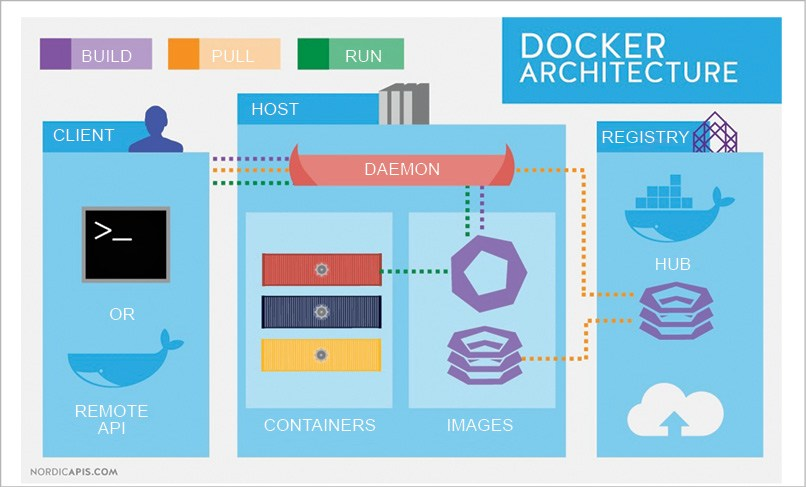
\includegraphics[scale=2]{Figure-1-Docker-container-architecture}
	\caption{Docker Architektur}
	\label{img:grafik-dummy}
\end{figure}
In Abbildung 1 sehen Sie die Hauptkomponenten einer Docker-Installation:
\begin{itemize}
	\item Im Zentrum steht der Docker-Daemon, der für das Erstellen, Ausführen und Überwachen von Containern sowie für das Erstellen und Speichern von Images zuständig ist. Der Docker-Dämon wird vom Host-Betriebssystem verwaltet.
    \item Der Docker-Client befindet sich auf der linken Seite und wird für die Kommunikation mit dem Docker-Daemon über HTTP verwendet. Ein Docker-Client kann mit mehr als einem Daemon kommunizieren, da sich der Docker-Client auf demselben Host wie der Daemon oder über eine Verbindung auf einem Remote-Host befinden kann. Der Docker-Client bietet eine Befehlszeilenschnittstelle (Command Line Interface, CLI), mit der Sie Anwendungsbefehle für einen Docker-Dämon erstellen, ausführen und stoppen können.
    \item Docker-Registrys speichern und verteilen images, die Standardregistrierung heißt Docker Hub und hostet Tausende von öffentlichen Images. Viele Unternehmen führen eigene Register, in denen kommerzielle oder vertrauliche Images gespeichert werden können. Der Docker-Daemon lädt als Reaktion auf Docker-Pull-Requests Images von Registrys herunter. Es werden auch automatisch Images heruntergeladen, die in Docker-Run-Requests und in der FROM-Anweisung von Dockerfiles angegeben sind, wenn sie nicht lokal verfügbar sind.
\end{itemize}
Wenn in diesem Abschnitt etwas nicht verstanden wird, wie z. B. Bilder, Dockerfile ..., machen Sie sich keine Sorgen, da in den folgenden Abschnitten alles im Detail erläutert wird.
\subsubsection{Docker Images}
\subsubsection{Docker Container}
\subsubsection{Docker Volumes}
\subsubsection{Data Container}
\subsubsection{Docker Compose}
\subsubsection{DockerFile}
\subsection{Git-Hosting mit Gogs}
\subsubsection{Einführung}
\subsubsection{Datenbankeinstellung}
\subsubsection{JGit}
\subsubsection{Webhook}
\section{Test-C Plattform}
\subsection{Einführung}
In diesem Abschnitt wird die Test C-Plattform detailliert beschrieben, wobei zunächst die Zusammensetzung der gesamten Programmarchitektur erörtert wird, anhand derer die Programmkomponenten separat diskutiert werden können. Nach der Erklärung der Komponenten des Programms auf separate Weise, wird im Abschnitt (Interne Prozesse) genau erläutert, wie sie zusammenarbeiten.
\newline
Wenn der Leser das oben Genannte versteht, kann er verstehen, was ich im Abschnitt  (Ablauf des Testverfahrens) erläutert wird.
\subsection{Architektur}
\begin{figure}[h!]
	\begin{center}
		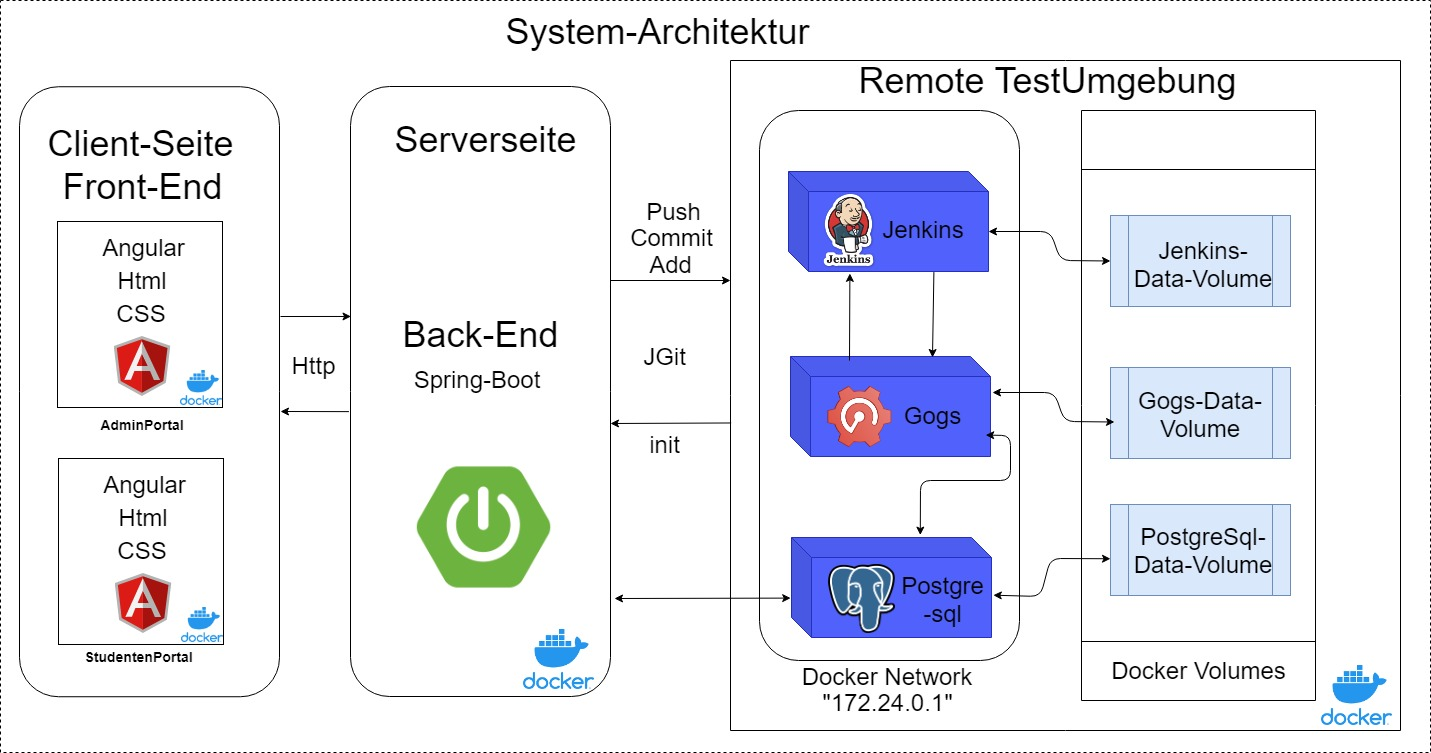
\includegraphics[width=17.5cm, height=13cm]{Test-C-Plattform-Arch.jpg}
		\caption{Architektur Test-C-Plattform } 
		\label{ Architektur Test-C-Plattform } 
	\end{center}
\end{figure}
Wie in der Abbildung 2 gezeigt, ist die Test-C-Plattformarchitektur in drei Hauptteile unterteilt: Client-Seite, Serverseite und Remote-TestUmgebung.
\newline
Die Wahl der Technologien beruhte auf ihrer Modernität und ihrer Verbreitung auf dem Arbeitsmarkt. In Teil eins des Projekts (Client-Seite/Frontend) wurde die folgenden Techniken verwendet : Angular 7, NGX-Bootstrap, Html, Css, im zweiten Teil des Projekts (Serverseite / BackEnd) wurden Maven und Spring Boot, Spring Security und Ldap ... verwendet. Der dritte Teil des Projekts, in dem der Testprozess durch Jenkins abgeschlossen ist.
\newline
Im folgenden Abschnitt werde ich jeden Teil des Architektur separat erklären.
\subsubsection{Client-Seite (Front-End)}
\begin{figure}[h!]
	\begin{center}
		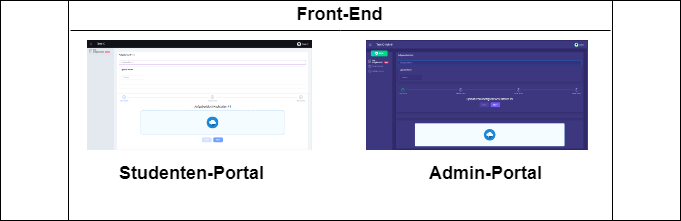
\includegraphics[width=17.5cm, height=7cm]{FrontEnd.png}
		\caption{Front-End } 
		\label{ Front-End } 
	\end{center}
\end{figure}
In diesem Projekt ist die Benutzeroberfläche in zwei Teile unterteilt: das Administrationsportal und das Studentenportal. Beide Portale wurden mit Angular 7, Html, Css und NGX-Bootstrap erstellt.
Über das Administrations Portal kann der Admin Benutzer ein neues Aufgabenblatt erstellen, dies bedeutet, dass ein virtueller Bereich für den Aufgabenblatttest erstellt wird, in dem die Studenten ihre Lösungen für Aufgaben testen können. Der Administrator kann alle Testdateien für jedes Aufgabenblatt in den entsprechenden Testbereich hochladen. Der Administrator kann auch die Testbereiche anzeigen. Jeder Testbereich ist mit dem Namen des zu testenden Aufgabenblatts gekennzeichnet. Für jeden Testbereich werden die spezifischen Testdateien angezeigt und der Administrator kann davon Dateien löschen oder andere hinzufügen.
Über das Studentenportal kann der Student die zu testende Lösungsdatei hochladen und dann an den Testbereich senden, der den Test automatisch durchführt und dem Studenten das Testergebnis anzeigt.
\subsubsection{Remote TestUmgebung}
Die Erklärung dieses Teils des Projekts vor der Erklärung des Mittelteils 'Serverseite' ist eine absichtliche Sache, damit der Leser einfach verstehen kann, was im Back-End passieren wird.
\newline
Die Remote-Testumgebung besteht aus drei miteinander verbundenen Docker-Containern (Jenkins-Container / Gogs-Container / PostgreSql-Container). Jeder Container verfügt über ein eigenes Datenvolumen zum Speichern der Daten. Dadurch wird vermieden, dass Informationen gelöscht werden, wenn der Container ausgeschaltet oder gelöscht wird.
\newline
Um einen Docker-Container in diesem Teil des Projekts zu erstellen, werden zwei verschiedene Methoden verwendet, entweder über eine Dockerfile Datei oder über eine Docker-Compose Datei.
\newline
Für den Jenkins-Container wurde eine Dockerfile Datei verwendet. Der Jenkins-Container besteht hauptsächlich aus einem Jenkins, den Compilern: gcc und g ++, die für den Build verantwortlich sind, und doxygen, das für den Testbericht verantwortlich ist.
\newline
Die Frage, die sich jetzt stellt, ist: Was ist eine Dockerfile Datei?
\newline
Ein Dockerfile ist einfach eine Textdatei mit einer Reihe von Anweisungen (instructions), die genutzt werden können, um ein Docker-Image zu erzeugen.
\newline
\begin{lstlisting}[caption=Dockerfile - jenkins]
FROM jenkins/jenkins

USER root

RUN apt-get -y update && apt-get -y upgrade

# install gcc g++ gfortran
RUN apt-get -y install build-essential

# install static analysis
RUN apt-get -y install doxygen graphviz
\end{lstlisting}
Die FROM-Anweisung legt fest, welches Basisimage zu verwenden ist, wie in diesem Fall Jenkins. RUN-Anweisunggen geben einen Schell-Befehl an, der im Image ausgeführt werden soll. In diesem Fall werden g++, gcc und doxygen ausgeführt.
\newline
Für den Gogs-Container und den PostgreSql-Container wurde eine Docker-Compose Datei verwendet.
Docker Compose wird zum Definieren und Ausführen von Docker-Anwendungen mit mehreren Containern verwendet. Mit Compose wird eine YAML-Datei (docker-compose.yml) verwendet, um die Dienste (services) von der Anwendung zu konfigurieren, wobei jeder Dienst (service) einen Container mit der zum Erstellen erforderlichen Konfiguration darstellt.
\begin{lstlisting}[caption=docker-compose.yml - Gogs/PostgreSql]
version: '2'
services:
app:
image: gogs/gogs:latest
volumes:
- /tmp/gogs-data:/data
ports:
- "3000:3000"
links:
- postgres:postgres
postgres:
image: postgres:alpine
volumes:
- /tmp/gogs-postgres:/var/lib/postgresql/data
environment:
- POSTGRES_USER=postgres
- POSTGRES_PASSWORD=password123
- POSTGRES_DB=gogs
\end{lstlisting}
Gogs ist ein einfacher selbst-gehosteter Git Service, der einfach einzurichten und zu betreiben ist und auf fast allem ausgeführt werden kann. Es ist zu Hundertprozent Open Source unter der MIT OSS-Lizenz. Gogs bietet die Anzeige und Bearbeitung von Repository-Dateien, die Verfolgung von Projektproblemen und ein eingebautes Wiki für die Projektdokumentation.
Gogs benötigt eine Datenbank, um den Quellcode zu speichern, daher wurde hier postgresql ausgewählt.
\newline
Nun stellt sich die Frage, wie die Container miteinander kommunizieren ?
\newline
Damit Docker-Container über den Host-Computer miteinander und mit der Außenwelt kommunizieren können, wird in diesem Fall eine Netzwerkschicht (Docker Networking) eingesetzt. Docker unterstützt verschiedene Arten von Netzwerken, die jeweils für bestimmte Anwendungsfälle geeignet sind: Bridge mode, Host mode, Container mode, und No networking.

\begin{lstlisting}[caption=Docker Network]
[
{
"Name": "gogs-compose_default",
"Id": "e19d76ee7d9f4132329d44e618bea3c5d93466527dd991d35b01fe4262ba6d73",
"Created": "2019-09-09T17:14:13.0772793Z",
"Scope": "local",
"Driver": "bridge",
"EnableIPv6": false,
"IPAM": {
"Driver": "default",
"Options": null,
"Config": [
{
"Subnet": "172.23.0.0/16",
"Gateway": "172.23.0.1"
}
]
},
"Internal": false,
"Attachable": false,
"Ingress": false,
"ConfigFrom": {
"Network": ""
},
"ConfigOnly": false,
"Containers": {
"0e69b0fffaf865665b4c2788f0d43a450301dff06ab1d50fedc4d24c0c97f0b4": {
"Name": "jenkins/jenkins",
"EndpointID": "0fc2f145af6d60b8da71e592299d9a0e2d7f578a392832baa0eb4f9e33b1c6e0",
"MacAddress": "02:42:ac:17:00:04",
"IPv4Address": "172.23.0.4/16",
"IPv6Address": ""
},
"264529e624168c9a64a308f2bbadeb26eb3676e54935de87f42675c114721754": {
"Name": "gogs-compose_app_1",
"EndpointID": "3309a74372ac94794dcf1e6f7df21cda2a54c1b98a608e3a5b9922098831d894",
"MacAddress": "02:42:ac:17:00:03",
"IPv4Address": "172.23.0.3/16",
"IPv6Address": ""
},
"6d04174448af71fd4a5de8735f5ad46e52145f933a3c5fbaa3ea53052eccf168": {
"Name": "gogs-compose_postgres_1",
"EndpointID": "e48d315587aa881a2d77984cb856a446d1c5fb74f6fa2f95bb3be6671b90dba7",
"MacAddress": "02:42:ac:17:00:02",
"IPv4Address": "172.23.0.2/16",
"IPv6Address": ""
}
},
"Options": {},
"Labels": {}
}
]
\end{lstlisting}


\subsubsection{Serverseite (Back-End)}
Nun wird über die Serverseite gesprochen, die für die Kommunikation des Benutzers mit der Testumgebung verantwortlich ist.
\newline
Die Serverseite stellt viele Dienste wie folgt bereit:
\paragraph{Benutzererkennung} In der westfälischen Hochschule Gelsenkirchen basiert die Speicherung der Hauptbenutzeridentitäten auf LDAP-Protokolls (Lightweight Directory Access Protocol) und gespeicherter LDAP-Datenbank. Dies hilft dabei, die Single Sign-On-Technologie (SSO) zu nutzen, die dadurch sich der Benutzer mit derselben ID und denselben Kennwörtern bei allen Anwendungen im selben Netzwerk anmelden kann. Um dies zu erreichen, sind 'spring-boot-starter-security' und 'spring-security-ldap' und 'unboundid-ldapsdk' in diesem Projekt verwendet.

\begin{lstlisting}[language=XML,caption=pom.xml - security dependencies]
<dependency>
<groupId>org.springframework.boot</groupId>
<artifactId>spring-boot-starter-security</artifactId>
</dependency>

<dependency>
<groupId>org.springframework.security</groupId>
<artifactId>spring-security-ldap</artifactId>
</dependency>
<dependency>
<groupId>com.unboundid</groupId>
<artifactId>unboundid-ldapsdk</artifactId>
</dependency>
<dependency>
<groupId>org.springframework.ldap</groupId>
<artifactId>spring-ldap-core</artifactId>
</dependency>
\end{lstlisting}
Unter Verwendung der obigen Abhängigkeiten werden Sicherheitsrichtlinienkonfigurationen wie folgt geschrieben: Zunächst wird festgelegt, welche Dienste der Benutzer ohne Anmeldung bereitstellen kann und bei welchen Diensten er sich anmelden muss. Wenn der Benutzer seinen Benutzernamen und sein Kennwort eingibt, wird überprüft, ob die Authentifikation-Daten gültig sind, indem sie mit den in der LDAP-Datenbank verfügbaren Daten verglichen werden.
\newline
Es wird nun davon ausgegangen, dass der Benutzer gültige Daten eingegeben hat. dh diese Daten sind identisch mit den in der LDAP-Datenbank gespeicherten Daten. Dann wird ein Token generiert und als Antwort auf die Authentifikation-Anfrage zurückgesendet. Dieses Token wird dann vom Frontend verwendet und mit jeder Anfrage gesendet.
\newline
Wird eine Anfrage geschickt, wird vom Backend dann überprüft, ob das Token gültig ist. Ist das der Fall, wird dann die Anfrage an den entsprechenden Controller weitergeleitet und damit die passende Funktion ausgeführt.

\paragraph{Erstellung eines neuen Aufgabenblatts}
Wie oben erklärt wurde, wird beim Erstellen eines neuen Aufgabenblatts ursprünglich ein neuer Testbereich erstellt, an dem die Studenten ihre Aufgabenlösungsdateien testen können. Mit anderen Worten, das Erstellen eines neuen Aufgabenblatts hängt vom Erstellen eines neuen Git-Repository ab, das denselben Namen wie das Aufgabenblatt hat z. B. (Aufgabenblatt-1) über die Gogs-Schnittstelle, die dem Administrator zur Verfügung steht und in der alle zum Testen erforderlichen Dateien gespeichert sind. Anschließend wird ein Jenkins Multibranch-Pipeline-Job erstellt, der auch denselben Namen wie das Aufgabenblatt hat.
\newline
Für die Erstellung von Multibranch-Pipeline-Job bietet Jenkins eine REST-API an, die viele Dienste bereitstellt, z. B. das Erstellen und Löschen von Job und viele andere Dinge. Um diese Jenkins-API zu verwenden, muss eine Maven-Abhängigkeit in pom.xml hinzugefügt werden.
\begin{lstlisting}[language=XML,caption=pom.xml - Jenkins-Api]
<dependency>
<groupId>com.offbytwo.jenkins</groupId>
<artifactId>jenkins-client</artifactId>
<version>0.3.7</version>
</dependency>
\end{lstlisting}
Zur Verdeutlichung wird erläutert, wie mit Jenkins-Api einen neuen Job erstellt werden kann. Um einen Job in Jenkins zu erstellen, müssen dem Job  ein Name und eine Reihe von Einstellungen nach Bedarf  zugewiesen werden.
\newline
Der Jobname wird als Zeichenfolge für die Jenkins-Api-Methode angegeben und die Einstellungen werden jedoch als XML-Datei dargestellt.
\begin{lstlisting}[language=JAVA,caption=JenkinsServiceImp - createJob]
@Override
public void createJob(String jobName, String jobXml) throws JenkinsException {
try{
JenkinsServer jenkinsServer = new JenkinsServer(new URI(jenkinsUrl), jenkinsUser, jenkinsPassword);
jenkinsServer.createJob(jobName, jobXml, true);
}catch (Exception e){
throw new JenkinsException(e);
} 
}
\end{lstlisting}
\paragraph{C-Datei-Upload}
Nachdem der Benutzer sein eigenes Konto erstellt und sich bei diesem Konto angemeldet hat, wird die zu testende Datei hochgeladen. Um diesen Service anbieten zu können, habe ich implementiert, was auf der Abbildung 4 gezeigt wird.
\begin{figure}[h!]
	\begin{center}
		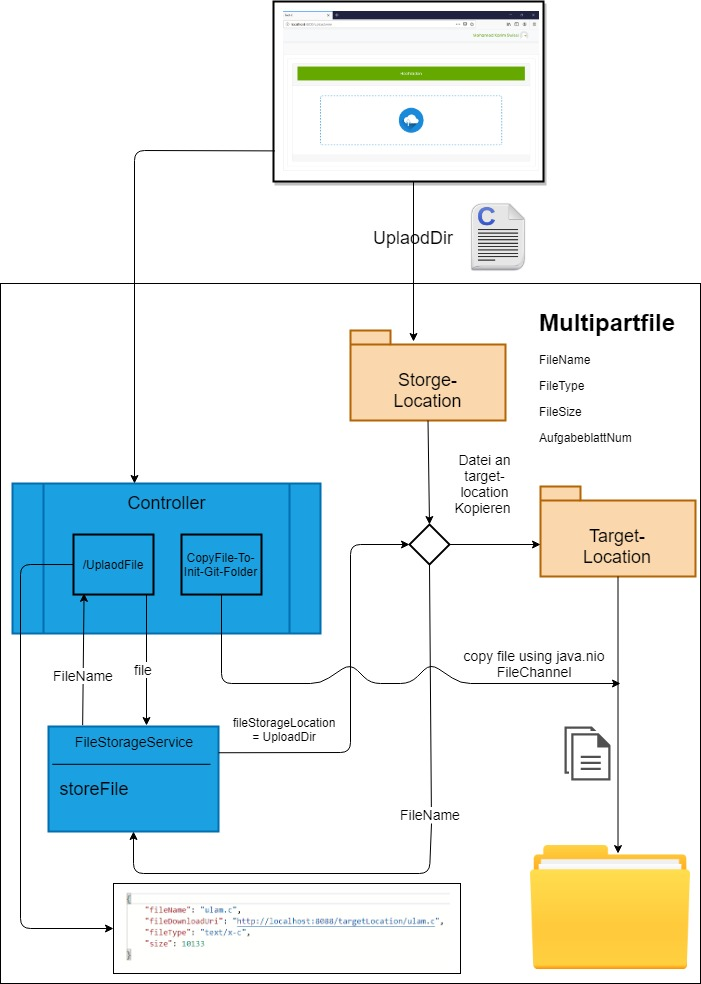
\includegraphics[width=17cm, height=17cm]{UplaodFileArchi.jpg}
		\caption{Back-End UplaodFile Architektur} 
		\label{Back-End UplaodFile Architektur} 
	\end{center}
\end{figure}
\newline
Das FrontEnd lädt eine C-Datei an einen temporären Speicherort im Speicher hoch. Darüber hinaus sendet das FrontEnd auch damit einige Informationen wie FileName und Aufgabenblatt-Nummer, daher empfängt das BackEnd die Datei in Form Multipartfile. Deshalb habe ich eine FileStorageProperties-Klasse erstellt, die als @ConfigurationProperties für die hochgeladene Datei festgelegt wird. Diese Klasse enthält als Attribute das Upload-Verzeichnis von der C-Datei und diese wird danach als fileStorageLocation Path missbraucht.
\begin{lstlisting}
@Autowired
public FileStorageService(FileStorageProperties fileStorageProperties) {
this.fileStorageLocation = Paths.get(fileStorageProperties.getUploadDir())
.toAbsolutePath().normalize();
}
\end{lstlisting}
Eine Post-Anfrage wird in dem Controller durch die Methode Uplaodfile generiert. Letzterere verwendet die in FileStorageService implementierte storeFile-Methode, um die Datei als Multipartfile  von fileStorageLocation nach targetLocation zu kopieren oder die vorhandene Datei mit demselben Namen zu ersetzen, dafür habe ich verwenden die abstrakte  Copy-Methode von java.nio.file.Files.
\begin{lstlisting}
 public String storeFile(MultipartFile file) {
// get File Name
String fileName = StringUtils.cleanPath(file.getOriginalFilename());

try {
// Ueberpruefen, ob der Dateiname ungueltige Zeichen enthaelt
if(fileName.contains("..")) {
throw new FileStorageException("Sorry! Filename contains invalid path sequence " + fileName);
}

// Datei an den targetlocation kopieren (Vorhandene Datei mit demselben Namen ersetzen)
Path targetLocation = this.fileStorageLocation.resolve(fileName);
Files.copy(file.getInputStream(), targetLocation, StandardCopyOption.REPLACE_EXISTING);

return fileName;
} catch (IOException ex) {
throw new FileStorageException("Could not store file " + fileName + ". Please try again!", ex);
}
}
\end{lstlisting}
Die UploadFile-Methode gibt ein UploadFileResponse-Objekt als Antwort zurück. Dieses enthält Informationen über die hochgeladene Datei, wie Dateiname und Aufgabenblattnummer.
\newline
Nachdem die zu testende C-Datei mit ihren Informationen als Multipartfile in TargetLocation verfügbar geworden ist, besteht der nächste Schritt darin, diese Datei an ein Initialisiertes Verzeichnis als Git-Repository kopieren.

\paragraph{Jgit-Operationen}


\subsubsection{Interne Prozesse}
\subsection{Alternativen}
\subsection{Ablauf des Testverfahrens}
\subsection{Installationsanleitung}
\subsection{Verwendung}
\section{Zusammenfassung}
\listoffigures
\section{Quellcodeverzeichnis}
\section{Quellenverzeichnis}
\end{document}